\chapter{Les travaux effectués et les apports du stage}
Au cours de ce stage, j'ai découvert le métier de consultant IT.
C'est un métier passionnant et varié.
Il requiert des capacités polyvalentes, du savoir-faire et de la flexibilité.

Les clients possédant chacun leur business, les problèmes qu'ils rencontrent ne sont jamais identiques.
Il faut donc maîtriser des connaissances dans plusieurs domaines et à plusieurs niveaux.
Avant d'être opérationnel, il faut posséder des connaissances théoriques et pratiques en infrastructure réseaux et en systèmes d'exploitation.

Certaines opérations ne peuvent se faire qu'en dehors des heures de bureaux, il est nécessaire de travailler parfois plus tard ou le weekend. 
D'autres ne se font que chez le client, il faut se déplacer jusque chez ce dernier.

En cas d'urgence ou d'incident grave, il faut être prêt à partir pour résoudre le problème du client. 

Pour des raisons propres à l'entreprise, il ne m'a pas été possible de travailler directement avec les clients.
Mais en me plaçant dans l'open space avec les consultants, il m'a été donné l'opportunité d'observer le travail de ces derniers dans la résolution des incidents.

\section{Travaux effectués}
Au cours de mon stage, mon travail a consisté essentiellement à réaliser l'architecture d'un laboratoire de test et à l'étude des connaissances relatives aux firewalls, passerelle SSL, tunnel VPN.

\subsection{Architecture du laboratoire de test}
Le laboratoire de la société permet aux employés de tester des nouvelles fonctionnalités, de simuler l'infrastructure d'un client afin de résoudre un problème, de configurer les machines à livrer à un client.
Sa disponibilité est capitale pour l'entreprise.

Le laboratoire possédait de vieux serveurs, qui n'étaient plus ou peu utilisés par manque de performance.
Les consultants travaillaient essentiellement avec cinq serveurs.
Ces serveurs faisaient tourner un système d'exploitation à la fois.
Il n'était pas évident de créer une infrastructure complète.
Ces cinq serveurs sont toujours opérationnels.
Nous avons remplacé uniquement les serveurs les plus anciens.

Le réseau de production est l'environnement de travail pour les techniciens. 
Sa structure est similaire à celle du laboratoire.
Il permet aux techniciens de se connecter à distance au réseau d'un client pour y procéder des maintenances, réaliser des interventions afin de résoudre un incident.

Avec l'arrivée des serveurs plus récents, l'utilisation du laboratoire est plus intéressante.
Il est désormais possible de créer une infrastructure complète en virtuel.
Les nouveaux serveurs possèdent entre seize (16) et vingt-quatre (24) gigaoctet (Go) de RAM.
Il est donc possible de faire tourner plusieurs machines virtuelles sur un même serveur physique.
Pour des raisons économiques, nous avons privilégié la solution de virtualisation de Windows, à savoir Hyper-V et la solution gratuite de VMWare, ESXi 5.5.

Les deux environnements de virtualisation ont des fonctions similaires.
Une différence à noter est que VMWare utilise un client pour la gestion de l'hôte physique alors que Hyper-V est un rôle à installer sur un serveur tournant sur Windows Server.  

\subsubsection{Matériel mis à disposition}
Le laboratoire est assez complet d'un point de vue matériel. 
Il est composé d'une quinzaine de serveurs dont des NAS, de plusieurs switchs, de multiples routeurs et firewalls, et de PDU (Power Distribution Unit).
Je met une liste du matériel hardware
\begin{itemize}
	\item Serveurs HP Proliant DL360 et DL380
	\item Switch Cisco 3560G, 2960G, 2950, 3750G
	\item Firewall Juniper NS25, SSG140, SRX240, SRX100
	\item Passerelle SSL SA2500
\end{itemize}
et une liste des systèmes d'exploitation et software sur lesquels j'ai travaillé
\begin{itemize}
	\item Windows Server 2008R2, 2012 et 2012R2
	\item Windows Client Vista, 7, 8 Professional et Enterprise
	\item ESXi 5.5
	\item ScreenOS 6.3r12
	\item JunOS 8.1r1.1
	\item Exchange 2013
	\item Office 2013
\end{itemize}

\subsubsection{Design du laboratoire}
Dans un premier temps, un collègue m'a présenté le schéma logique du nouveau plan du laboratoire.
Sur base de ce plan, nous avons exploré l'ensemble des technologies à mettre en place.
Ce plan prévoyait la création de deux sous-réseaux à l'intérieur du réseau de laboratoire.
Pour créer ces sous-réseaux, nous avons configuré deux firewalls NetScreen 25 de Juniper. 
Il prévoyait également des connexions iSCSI entre les serveurs et les disques virtuels de stockage sur les NAS.

Le laboratoire est composé de quatre racks, le rack 4 est réservé aux connexions vers la salle de production et vers l'open-space.
Nous avons décidé de placer les serveurs dans le rack 1 et le matériel réseau dans le rack 2.
Le rack 3 contient des Access Point pour le labo et accueille une solution Voice de Cisco depuis peu.

\subsubsection{(Dés)Installation des serveurs}
Nous avons commencé par enlever les anciens serveurs.
Ensuite, nous avons récupéré les nouveaux serveurs, que nous avons entreposés en attendant un plan détaillé de la localisation de ces derniers.

Pour établir la disposition exacte des serveurs, nous avons relevé les composants de tous les serveurs.
Nous avons pris note du nombre de cœurs physiques, de la quantité de RAM ainsi que de la disposition des slots de RAM.
Pour les disques durs, nous avons regardé au RAID formé, ainsi que la capacité de chaque disque.

Ensuite, nous avons classé les serveurs du plus puissant au moins performant. 
Les six serveurs les plus puissants sont configurés comme host de machine virtuelle. 
Quatre tournent sous Windows 2012R2 Datacenter avec le rôle Hyper-V et les deux autres tournent sous ESXi 5.5.
Parmi les autres serveurs, nous en avons choisi un pour faire tourner uniquement le service WSUS (Windows Server Update Services) sur un Windows Server 2012R2. 
Ce service permet de mettre à jour toutes les machines Windows qui s'y connectent.
Il télécharge les mises à jour depuis le serveur de Microsoft et est capable de les déployer sur les machines locales.
Cet outil est utile quand il y a beaucoup de machines sur le réseau à mettre à jour. 

\subsubsection{Connexion des serveurs}
Pour les serveurs, les manipulations étaient simples. 
Il suffisait de débrancher tous les câbles du serveur.
Ensuite de l'enlever des rails et d'enlever ces derniers du rack pour récupérer l'espace.
Pour placer les nouveaux, nous placions le rail en premier, puis le serveur dessus.
Le câblage des serveurs s'est fait un peu plus tard, car nous devions vérifier le nombre de connecteurs réseau. 

En effet, nous avons créé des EtherChannel quand c'était possible.
Pour créer les EtherChannel, nous avons configuré le NIC Teaming sur les serveurs en mode LACP.
Nous avons aussi configuré les ports sur le switch afin de gérer les EtherChannel.
 
Nous avons besoin d'une grande bande passante entre nos serveurs et nos NAS (Network-Attached Storage) pour réduire les temps de transfert des VM (Virtual Machines).
Nous avons profité du fait que le switch principal a tous ses ports en gigabit. 
Ainsi, nous avons au minimum 1Gbps de vitesse de transfert et grâce au EtherChannel, nous montons jusqu'à 4Gbps.
Nous stockons les VMs sur les NAS, et chaque serveur possède une connexion iSCSI vers un iSCSI Target. 

L'avantage d'utiliser Windows 2012 R2 est que le NIC Teaming peut se faire via le Server Manager alors que dans les anciennes versions, il fallait utiliser le software du fabricant.


Pour le câblage, nous avons utilisé les bonnes pratiques en "cable management" :  
\begin{itemize}
\item Tous les câbles sont étiquetés aux deux extrémités
\item Utilisation d'un code couleur pour les différents types de câbles
\item Séparation physique entre les câbles Ethernet et les câbles d'alimentation
\item Emploi de câbles de bonnes longueurs
\end{itemize}

\subsubsection{Switch KVM}
Un switch KVM (Keyboard, video and mouse) est installé dans le rack.
Il nous permet de contrôler un serveur à distance comme si nous étions dessus en physique.
Il simule le clavier, l'écran et la souris sur le serveur. 

\subsubsection{Solution VoIP}
Par la suite, nous avons reçu un solution complète de Voice.
Cette solution est composée d'un serveur, de six routeurs et six switchs.
Il permet de créer une infrastructure Voice d'une entreprise.

\subsubsection{Partie software}
Comme dit au point précédent, certains serveurs sont des hôtes pour des VMs.
J'ai donc installé des serveurs Windows 2012 R2, ainsi que des ESXi 5.5.

Les serveurs n'étant plus à jour, une mise à jour des drivers était nécessaire surtout pour les machines passant à un Windows Server 2012R2.
Les mises à jour ont été effectuées à l'aide d'une WebApp de HP.

Le laboratoire ne gère pas les domaines Active Directory, car son fonctionnement n'est pas compatible avec l'utilisation que l'on fait du labo. 
Les machines que nous installons, en virtuel ou physiquement, ont des durées de vie limitées.
Elles restent actives entre une semaine et un mois.

\subsubsection{Plan d'adressage}
Sur base du classement, j'ai aussi défini le plan d'adressage des serveurs (voir Tab.\ref{tab:addIP} p.\pageref{tab:addIP}).
Même si la plupart des serveurs possèdent plusieurs cartes réseaux, ils n'ont qu'une seule adresse IP attribuée.
En effet, nous avons utilisé du NIC Teaming pour regrouper les interfaces physiques en un seul interface logique.
Il y a juste les serveurs ESXi qui ont deux adresses IP : la première sert au management et la deuxième permet les connexions iSCSI.
Cette séparation n'est pas nécessaire, mais elle est conseillée.
\begin{table}
\centering
\begin{tabular}{cc}
\toprule
Nom du serveur & Adresse IP \\
\midrule
HV-01 & 192.168.6.10 \\ 
HV-02 & 192.168.6.11 \\ 
ESXi-01 & 192.168.6.12 (Mgmt) - 192.168.6.21 (iSCSI) \\ 
ESXi-02 & 192.168.6.13 (Mgmt) - 192.168.6.20 (iSCSI) \\ 
HV-03 & 192.168.6.14 \\ 
HV-04 & 192.168.6.15 \\ 
WSUS & 192.168.6.16 \\ 
HP-NAS-01 & 192.168.6.17 \\ 
HP-NAS-02 & 192.168.6.18 \\ 
HP-NAS-03 & 192.168.6.19 \\
\bottomrule
\end{tabular}
\caption{Adressage des serveurs du laboratoire}
\label{tab:addIP}
\end{table}

Une fois les systèmes d'exploitation installés et les adresses configurées, tous les serveurs sont accessibles en remote. 

\subsection{Rôles des serveurs}
Nous avons installé les rôles Hyper-V sur les quatre serveurs dédiés, et nous avons configuré les iSCSI Initiator. 
Le role Hyper-V permet de manager des machines virtuelles. 
C'est une solution Windows, elle ne fonctionne qu'avec des VHD (Virtual Hard Disk). 

ESXi est la solution gratuite de virtualisation de VMWare. 
Pour manager les VMs, le client vSphere Hypervisor doit être installé sur une machine.

\subsection{Réglage du WSUS}
Le serveur WSUS fonctionnait correctement.
Mais pour le rendre accessible aux machines, nous avons dû modifier une valeur du registre windows.
Ce changement de valeur est à réaliser sur toutes les machines qui vont utiliser le serveur WSUS.
Nous avons créé un fichier contenant les modifications à effectuer.
Nous l'avons sauvegardé au format \texttt{.reg}.
Finalement, nous l'avons copié et exécuté sur les machines concernées. 
Cette modification a pour but d'obliger la machine à contacter le serveur WSUS interne plutôt que le serveur Microsoft. 

\subsection{Templates Windows}
Il m'a été demandé de créer des \textit{templates} des systèmes d'exploitations.
Ces \textit{templates} ont pour objectif de fournir des systèmes pré-installés que nous pouvons déployer directement.

La création de ces derniers est simple. 
La procédure décrite ci-dessous est celle de la société.
Il suffit de posséder une image du système d'exploitation.
Ensuite, nous démarrons la VM pour l'installation de base. 
Dès que le système est installé, nous avons appliqué toutes les mises à jour requises depuis le serveur WSUS. 
Finalement, nous avons exécuté la commande \texttt{sysprep} dans le \textit{cmd}.
Cette commande modifie des valeurs uniques créées par le système.
Par exemple, deux serveurs issus du même \textit{template} sans avoir lancé la commande \texttt{sysprep} ne peuvent pas être dans le même domaine, car ils possèdent des identifiants identiques. 

\section{Lien avec le TFE}
Mon sujet de TFE a été choisi en accord avec la société.
Le TFE porte sur les accès distants.
Il requiert l'utilisation de firewall, de passerelle SSL.
Il repose sur un environnement professionnel.
Il a été nécessaire de créer cet environnement, qui consiste en un domaine Active Directory et un serveur Exchange. 
De plus, un ordinateur interne au domaine servait pour les tests de connectivité.
Par la suite, cet ordinateur se connectait depuis un réseau externe à celui du domaine pour simuler l'accès distant.

Grâce à l'architecture du laboratoire, l'environnement de test pour mon TFE était réalisable sans pénaliser mes collègues.
Mon environnement se compose de trois serveurs sous \textit{Windows 2012 R2} et d'un ordinateur sous \textit{Windows 8.1 Enterprise}.
Il m'a été fourni le matériel nécessaire à la réalisation de cette infrastructure.
 

\section{Fait Marquant}
Lors des tests de l'infrastructure de mon TFE, nous sommes tombés sur un problème de connectivité entre une machine distante et un serveur Exchange interne via un tunnel VPN. 
Ce problème s'était posé chez un client et était en cours de traitement par l'un de mes collègues.
Le fait d'avoir pu recréer cet incident, nous a permis de fournir une solution au client concerné. 
Comme nous possédions une infrastructure similaire, nous avons pu mener un ensemble de tests afin de déterminer le problème.
Nous avons commencé par vérifier l'état du tunnel VPN.
Tout semblait correct, la connexion s'établissait dans le mode ESP.
Et si cette connexion échouait pour une raison quelconque, le système essayait d'établir la connexion en SSL.
En réalisant des tests de connexion-déconnexion, nous nous sommes rendus compte que le problème résidait dans l'option de fallback entre l'ESP et le SSL.
La cause du problème n'est pas de notre ressort, car elle nous semblait venir d'une incompréhension dans le DNS du client Windows.
\begin{figure}[!h]
\centering
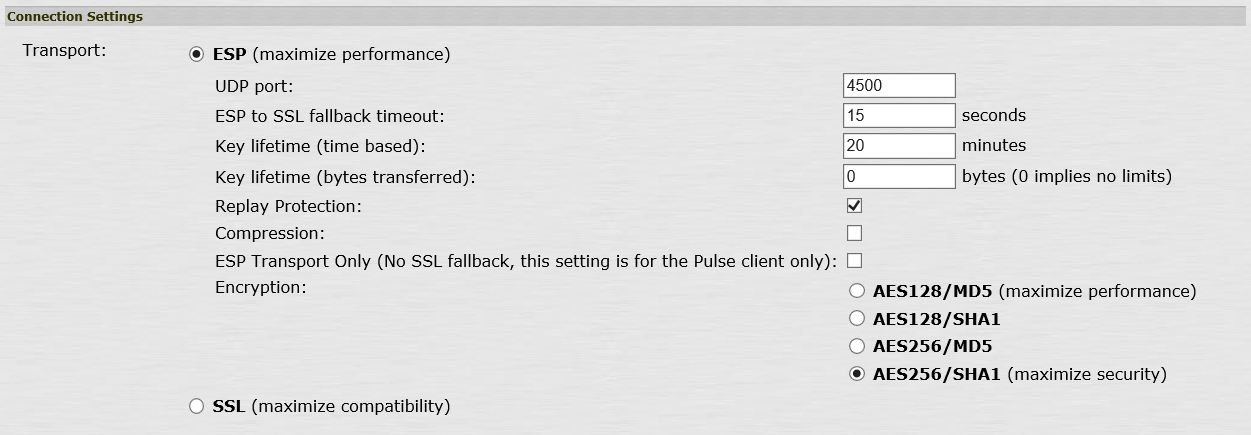
\includegraphics[width=16cm]{fallbabkssl.png}
\caption{Les modes de tunnel de Pulse Secure}
\label{fig:ssl}
\end{figure}
La figure \ref{fig:ssl} montre les modes de tunnel et les options associées.
Pour vérifier notre hypothèse, nous avons mené des tests en désactivant l'option de fallback.
Nous avons alors forcé le tunnel ESP en ajoutant une règle dans le firewall qui autorise l'utilisation du port 4500 sur la passerelle.
Ensuite, nous avons recommencé les tests de connexion-déconnexion, et nous avons prouvé que le problème avait disparu.
Par contre, cette solution n'est pas optimale car l'utilisation de ESP n'est pas possible pour des appareils mobiles de types smartphones.
Afin de ne pas créer un nouvel incident, nous sommes passés à des tunnels SSL. 

\section{Apports du stage}
J'ai appris énormément de choses pendant ces quatorze semaines de stage aussi bien d'un point de vue technique que humain.

\subsection{Compétences théoriques acquises}
L'apprentissage des technologies passe par une phase d'étude, puis par la pratique.
J'ai passé un certain temps à étudier le fonctionnement de divers protocoles liés à la sécurité des données tels que IPSec et SSL/TLS.
De plus, j'ai du m'habituer aux termes techniques utilisés au sein de la société.

\subsection{Compétences techniques acquises}
Lors de ce stage, j'ai appris à installer des serveurs en suivant de bonnes pratiques, à concevoir un laboratoire en respectant les règles de "cable management", à configurer des firewalls, des switchs, des passerelles SSL. 

Dans les points suivants, je décris les technologies utilisées, ainsi que certaines bonnes pratiques apprises.
Il me semble utile de commencer par la base d'une infrastructure.
Par la suite, il est intéressant d'expliquer des éléments plus techniques tels que un firewall et une passerelle SSL. 
\subsubsection{Infrastructure Windows}
Une infrastructure professionnelle en Windows possède au minimum un serveur Active Directory (AD) avec le rôle Domain Controller (DC) et un serveur Exchange. 
L'utilisation d'Exchange requiert l'utilisation de certificats, il est donc nécessaire d'ajouter le rôle Certificate Services (CS) à l'AD.

La gestion des certificats est un peu complexe au premier abord.
Un collègue a pris le temps de m'expliquer le rôle d'une autorité de certification (CA) et comment créer une requête pour un serveur auprès du CA. 

Pour le stockage entre les serveurs et les NAS, la meilleure solution consiste à utiliser des disques iSCSI.
La nomenclature iSCSI est assez lourde, mais son fonctionnement est simple. 
Il suffit de créer un espace de stockage dynamique ou statique que l'on associe comme iSCSI Target. 
Ensuite, les clients, appelés iSCSI Initiator, se connectent aux disques cibles. 
Selon les autorisations, l'accès est accepté ou refusé.
L'avantage d'un disque iSCSI est qu'il est visible par le système d'exploitation de la même façon qu'un disque local. 

\subsubsection{Firewall Juniper}
Une notion essentielle de la gestion des firewalls Juniper est celle de Virtual Router.
Dans un firewall Juniper, les zones de confiance et les zones de non-confiance sont isolées l'une de l'autre.
C'est comme si on avait deux routeurs connectés l'un à l'autre dont l'un distribue les routes pour la zone de confiance et l'autre fait de même pour les zones de non-confiance.
Pour que du trafic passe entre les deux routeurs, les routes doivent être configurées manuellement.

En plus des routes, les firewalls se basent sur l'utilisation de Policies pour filtrer le trafic.
Les policies fonctionnent soit avec des adresses IP, soit avec des objets. 
Il est conseillé d'utiliser les objets, car ils masquent les adresses IP associées. 
Ainsi, lors d'un changement d'adressage, il suffit de modifier les propriétés de l'objet plutôt que d'aller modifier toutes les policies impactées.
\subsubsection{Passerelle SSL}
Une passerelle SSL gère les connexions distantes.
Elle dispose d'un ensemble de règles d'authentification et d'accès pour autoriser ou non une connexion distante.

\subsubsection{EtherChannel}
L'EtherChannel permet d'assembler d'un point de vue logique plusieurs ports d'un switch pour n'en former qu'un.
L'un des avantages est une plus grande bande passante, car chaque lien est indépendant de l'autre.
Ainsi, le système peut utiliser tous les liens pour l'envoi de données ou la réception ou faire un mix entre les deux en fonction de la charge. \\

Ces connaissances m'ont été utiles pour mon travail de fin d'études. 

\subsection{Difficultés rencontrées}
Dans un premier temps, les problèmes étaient surtout d'un niveau théorique vu que je ne connaissais pas toutes les technologies à mettre en place. Avec le temps, ce genre de problème est devenu de plus en plus rare.
Par contre, les problèmes de configuration et de matériel sont devenus plus fréquents.
Par la pratique, certaines difficultés ont disparu ou sont devenues évitables. 

\subsection{La vie en société}
Travailler dans une PME a des avantages pour les relations humaines.
Il est en effet plus facile de discuter avec l'ensemble des employés.

Mon intégration s'est bien déroulée. 
Ma place dans l'open space m'a permis de côtoyer mes collègues en permanence.
Mon bureau était à côté de celui d'un technicien et en face du commerciale.
Il y avait toujours au moins un technicien au bureau pour répondre à la hotline.
De ce fait, il y avait quelqu'un pour répondre à mes questions. 

Mes collègues étant assez jeunes, moins de 40 ans.
Il ne m'a pas été trop difficile de m'entendre avec eux.
De plus notre passion pour l'informatique aide pour discuter des nouveautés ou des technologies plus anciennes.

\'Evidemment, je ne les ai pas aidées dans leur tâches.
Mais pour toutes questions relatives au laboratoire, j'étais la personne à questionner. 
Les discussions dans l'open space m'ont permis d'apprendre sur le fonctionnement de l'entreprise et sur la réalité du travail en temps que consultant.

Au début, il m'a été assigné un collègue qui servait de point de contact lorsque j'avais une question.
Mais le métier de consultant implique de se déplacer soit chez un client, soit dans un centre de formation, soit en urgence.
Il est arrivé que ce collègue parte en milieu de journée ou qu'il soit absent une semaine complète pour donner un cours.
Au lieu de perdre mon temps, j'ai demandé des conseils aux autres collègues présents au bureau.
C'est ainsi que j'ai remarqué le niveau de compétence de l'ensemble des consultants.

L'ambiance au bureau était bonne, nous pouvions avoir des moments de rigolade, et aussi des moments de travail au calme.

